\documentclass{article}

\usepackage{arxiv}

\usepackage[utf8]{inputenc} % allow utf-8 input
\usepackage[T1]{fontenc}    % use 8-bit T1 fonts
\usepackage{hyperref}       % hyperlinks
\usepackage{url}            % simple URL typesetting
\usepackage{booktabs}       % professional-quality tables
\usepackage{amsfonts}       % blackboard math symbols
\usepackage{nicefrac}       % compact symbols for 1/2, etc.
\usepackage{microtype}      % microtypography
\usepackage{lipsum}		% Can be removed after putting your text content
\usepackage{amssymb,amsmath,amsthm}
\usepackage{listings}
\usepackage{graphicx}
\usepackage{subfig}
\usepackage{apacite}
\usepackage{algorithm}
\usepackage{algorithmicx}
\usepackage{algpseudocode}
\usepackage{kbordermatrix}% http://www.hss.caltech.edu/~kcb/TeX/kbordermatrix.sty
\usepackage{todonotes}
\usepackage{natbib}

\newtheorem{theorem}{Theorem}
\DeclareMathOperator\supp{supp}

\title{Data assimilation with agent-based models using Markov chain sampling}

%\date{September 9, 1985}	% Here you can change the date presented in the paper title
%\date{} 					% Or removing it

\author{
  Daniel Tang\\
    Leeds Institute for Data Analytics, University of Leeds, UK\thanks{This project has received funding from the European Research Council (ERC) under the European Union’s Horizon 2020 research and innovation programme (grant agreement No. 757455)}\\
  \texttt{D.Tang@leeds.ac.uk}\\
  \AND
  Nick Malleson\\
  School of Geography, University of Leeds, UK\\  
  %% examples of more authors
  %% \AND
  %% Coauthor \\
  %% Affiliation \\
  %% Address \\
}


\begin{document}
\maketitle

\begin{abstract}
Every day, weather forecasting centres around the world receive noisy, incomplete observations of the atmosphere and use this data to update the state of their atmospheric models and forecasts. This process is known as data assimilation, data fusion or state estimation and is best expressed as Bayesian inference: given a set of observations, some prior beliefs and a model of the target system, what is the probability distribution of some set of unobserved measures at some time, possibly in the future?

While data assimilation has developed rapidly in some areas of application, relatively little progress has been made in performing data assimilation with agent based models. This has hampered the use of agent based models to make quantitative claims about real-world systems.

Here we present an algorithm that uses Markov-Chain-Monte-Carlo methods to generate samples of the trajectories of an agent based model over a window of time given a set of noisy, incomplete observations of the system. This approach is more likely to be a feasible means of assimilating observations than the current state-of-the-art (that typically involves trying to apply existing data assimilation methods such as those used in weather forecasting to an agent-based model directly). 

The algorithm is applicable to time-stepping agent based models whose agents have a finite set of states and a finite number of ways of acting on the world. As presented the algorithm is only practical for agents with a few bytes of internal state although we discuss ways of removing this restriction. We demonstrate the algorithm by performing data assimilation with an agent-based, spatial predator-prey model.
\end{abstract}

% keywords can be removed
\keywords{Data assimilation, Bayesian inference, Agent based model, Integer linear programming, predator prey model}

\section*{Minor things}
\begin{itemize}
	\item Replace 'agent based' with 'agent-based' to be consistent
\end{itemize}

\section{Introduction}

Agent-based models (ABMs) have been widely adopted as an intuitive way to model systems that consist of a heterogeneous collection of autonomous, interacting agents. The uses of ABMs can be broadly be divided into two categories. \textit{Abstract} models are typically used to explore the fundamental dynamics of a system. For example, \citet{schelling1971dynamic} famously showed that an unexpected collective behaviour can emerge from a known agent behaviour; agents with only a very slight preference to live close to agents of their own race can quickly form a highly racially-segregated population. This use of ABMs requires no assimilation of real-world data but as a consequence the model's output cannot be used to make direct assertions about the real world. \citeauthor{schelling1971dynamic}'s model \textit{might} reveal something about the dynamics of real human patterns in segregation, but to be sure we need to first demonstrate that the model is a proper abstraction of the real-world. \textit{Predictive} ABMs, on the other hand, are those that use real-world observations to demonstrate that that they are reliable abstractions and hence can be used to make predictions about current or future system states. In this paper we'll deal with the `predictive' case, where we have an ABM of some real-world target system and some observations of that same system. Our aim will be to combine the information in the observational data with the knowledge encoded in the model to learn something about some set of unobserved real-world measures.

XXXX HERE - summarise paper method and results.

The paper is structured as follows: Section~\ref{sec:context} discusses the context and related research; Section~\ref{sec:formulation} formulates the problem in detail; Sections~\ref{sec:approx_support} and~\ref{sec:posterior_sampling} outline the method; Section~\ref{sec:demonstration} demonstrates the algorithm in the context of a predator-prey model; Sections~\ref{discussion} and~\ref{sec:conclusion} provide the discussion and conclusions.


\section{Context and Literature Review}\label{sec:context}

This section will outline the problem with more detail and the drawbacks with the state-of-the-art approaches. Recall that our aim is to combine sparse observational data with an uncertain agent-based model to generate a more realistic picture of the true state of a system than would be possible with the observations or the model in isolation. The observations may contain aggregated or macro-scale measures and may be subject to noise during the measurement process. The unobserved measures may be taken at any time, and may include times before, during and/or after the observed interval. The behaviour of the agents in the model will generally be stochastic, in order to account for our uncertainty in agent behaviour, and will be a function of some set of unknown parameters, $\theta$, in order to account for our uncertainty over which behavioural model best represents the real-world target entities, or over the values of measures that we know are constant over time. Note that the parameters can, and generally should, contain values that control the size of the model stochasticity in order to account for ``unknown unknowns''. The target system may also interact with a world outside of the model, these interactions necessarily consist of agents being injected into the model at certain times and/or external influences on modelled agents' behaviour\footnote{we take the purist view that an ABM models everything as an agent}. The start state of the model is also a boundary condition, consisting of the injection of agents into the model at time $t=0$. Although the boundary conditions are semantically distinct from the parameters, their mathematical treatment will be identical so we assume $\theta$ includes any boundary conditions. So, an ABM defines a distribution, $P(\tau| \theta)$, which is the probability that the agents would exhibit behaviours $\tau$ on a model execution with parameters/boundary conditions $\theta$. We'll call $\tau$ a \textit{model trajectory}.

Letting $\Omega$ be our set of real-world observations, our aim can be expressed as the approximation of the expectation of some arbitrary unobserved measure, $\Lambda$, given the observations
\begin{equation}
\mathbb{E}_{P(\tau,\theta|\Omega)}(\Lambda(\tau,\theta)) = \int \Lambda(\tau,\theta) P(\tau,\theta|\Omega) d\tau d\theta
\label{expectation}
\end{equation}
This assumes that $\Lambda$ can be calculated from the model trajectory, the parameters and the boundary conditions\footnote{If this isn't the case then we're simply using the wrong model for our needs}. 

There are various strategies to solve this equation for ABMs. One strategy is to first transform the ABM into a simpler form, such as a set of partial differential equations \citep{lloyd_exploring_2016} or a graphical model \citep{liao2010integrated}, for which there exists a well known method of solving the problem. An alternative strategy is presented in \citet{tang2019data} where creation and annihilation operators are employed to describe an ABM and the integral in \eqref{expectation} is calculated using symbolic computation. However, the most popular strategy is to approximate $\mathbb{E}_{P(\tau,\theta|\Omega)}(\Lambda(\tau,\theta))$ by sampling from the posterior $P(\tau,\theta|Omega)$ and using Monte Carlo integration, this is the technique we employ here.

Bayes' rule gives us
\begin{equation}
\mathbb{E}_{P(\tau,\theta|\Omega)}(\Lambda(\tau,\theta)) = \int \Lambda(\tau,\theta) \frac{P(\Omega|\tau)P(\tau|\theta)P(\theta)}{P(\Omega)} d\tau d\theta
\label{bayesassimilation}
\end{equation}
where $P(\theta)$ is our prior belief about the parameters and boundary conditions (after accounting for any micro-calibration data or other relevant direct observations we may have), $P(\tau|\theta)$ is our ABM and $P(\Omega|\tau)$ is the probability of making observations $\Omega$ given the trajectory. We assume this is easy to calculate given a trajectory that covers the observed period. The prior probability of the observations, $P(\Omega)$, is just a normalising constant so is not usually explicitly calculated when sampling.

Once expressed in this form we can, in theory at least, approximate $\mathbb{E}_{P(\tau,\theta|\Omega)}(\Lambda(\tau,\theta))$ using importance sampling as follows:
\begin{enumerate}
\item Take a sample from the prior parameters and boundary conditions $\theta_i \sim P(\theta)$.
\item Execute the model forward with parameters $\theta_i$ to generate a sample trajectory $\tau_{i} \sim P(\tau|\theta_i)$.
\item Calculate a weight $w_i = P(\Omega|\tau_i)$ to create a weighted sample $\left<\tau_{i},\theta_i, w_i\right>$.
\item Repeat  N times from step 1 to get a set of weighted samples $\left\{\left<\tau_1,\theta_1,w_1\right> \dots \left<\tau_N,\theta_N,w_N\right> \right\}$.
\item Approximate $\mathbb{E}_{P(\tau,\theta|\Omega)}(\Lambda(\tau,\theta)) \approx \sum_{i=1}^N \frac{w_i\Lambda(\tau_i,\theta_i) }{\sum_{j=1}^Nw_j}$
\end{enumerate}

However, \citet{chatterjee2018sample} show that the information contained in the weighted samples reduces exponentially with the KL-divergence from the prior to the posterior, $D_{KL}\left(P(\tau,\theta|\Omega) \mid\mid P(\tau|\theta)P(\theta) \right)$. This divergence can be thought of as a measure of the information in the observations $\Omega$. In practice, in the case of ABMs, the observations usually contain enough information to make the set of weighted samples less informative than a single unweighted sample, even when $N$ is astronomically high. So this algorithm will not work.

A popular strategy to tackle this problem is to split the time period we're interested in into smaller, contiguous time windows with (not necessarily equidistant) end times $\left<t_1 \dots t_N\right>$ where $t_m < t_{m+1}$. The trajectory and observations can be similarly split based on which window they occur in, $\tau = \left<\tau_1 \dots \tau_N\right>$ and $\Omega = \left<\Omega_1 \dots \Omega_N\right>$. The posterior distribution of the whole trajectory can then be split into the product of contributions from each window given the end state from the previous window, leading to a recursion relation
\begin{equation}
P\left(\tau_{1:t+1}, \theta | \Omega_{1:t+1}\right)
=
\frac{ P(\Omega_{t+1}|\tau_{t+1})
P(\tau_{t+1}|\tau_{1:t},\theta) P\left(\tau_{1:t},\theta| \Omega_{1:t}\right)
}
{	P(\Omega_{t+1}| \Omega_{1:t}) }
\label{bayesrecursion}
\end{equation}
where $\tau_{1:t} = \left<\tau_1 \dots \tau_t\right>$ and $P(\tau_{t+1}|\tau_{1:t},\theta)$ is the probability that an execution of the ABM that starts with trajectory $\tau_{1:t}$ would go on to produce $\tau_{t+1}$ given the parameters/boundary conditions $\theta$. The final posterior $P(\tau_{1:N},\theta|\Omega_{1:N})$ can now be built up in steps, starting with the first window and moving to the last, using the recursion as we go. This makes the problem easier in two respects, firstly the dimension of the distributions we need to deal with at each recursion step are reduced since we're only concerned with the trajectory in one window at a time, secondly we split the information in the observations into smaller chunks, so at each recursion the information in $\Omega_t$ is more likely to be small enough to make it practical to perform importance sampling with the prior. This describes the \textit{particle filtering} or \textit{sequential Monte Carlo} approach to Bayesian inference.

If the unobserved measure of interest, $\Lambda$, depends only on the states of the agents, $\sigma_N$, at time $t^N$ and/or the parameters/boundary conditions, $\theta$, rather than on the full trajectory, $\tau_{1:N}$, then we can reduce the dimensionality even further by performing the recursion on model states rather than trajectories (where a model state tells us how many agents there are in each agent state). First arrange the windows so that each observation lies at the end of a window, then marginalise equation \eqref{bayesrecursion} over $\tau_{1:t+1}$ for a fixed $\sigma_{t+1}$ to get
\begin{equation}
P\left(\sigma_{t+1}, \theta | \Omega_{1:t+1}\right)
=
\frac{ P(\Omega_{t+1}|\sigma_{t+1}) 
}
{	P(\Omega_{t+1}| \Omega_{1:t}) }
\int P(\sigma_{t+1}|\sigma_t,\theta)P\left(\sigma_{t},\theta| \Omega_{1:t}\right) d \sigma_t
\label{bayesstaterecursion}
\end{equation}
where we've assumed that the observation likelihoods depend only on the model state and made explicit in $P(\sigma_{t+1}|\sigma_t,\theta)$ that the probability of the state $\sigma_{t+1}$ depends only on $\sigma_t$ and $\theta$  \footnote{technically, if $\theta$ contains time dependent boundary conditions, the model states need to be timestamped so that the model knows which boundary conditions to apply}.   Note that the definition of ``model state'' can always be re-defined in such a way as to make these assumptions true. In fact, we can see that equation \eqref{bayesrecursion} can be thought of as a special case of equation \eqref{bayesstaterecursion} where the model state, $\sigma_t$, is the trajectory, $\tau_{1:t}$, and the integral over $\sigma_t$ is non-zero for only a single trajectory, since $P(\tau'_{1:t+1}|\tau_{1:t},\theta) = \delta_{\tau'_{1:t}}(\tau_{1:t})P(\tau'_{t+1}|\tau_{1:t},\theta)$, where $\delta$ is the delta distribution.

So, we can consider a recursion on \textit{generalised trajectories}, $T_t$,
\begin{equation}
P\left(T_{t+1}| \Omega_{1:t+1}\right)
=
\frac{ P(\Omega_{t+1}|T_{t+1})}
{	P(\Omega_{t+1}| \Omega_{1:t}) }
\int P(T_{t+1}|T_t)P\left(T_{t}| \Omega_{1:t}\right) d T_t
\label{generalisedbayesrecursion}
\end{equation}
so that equations \eqref{bayesrecursion} and \eqref{bayesstaterecursion} would correspond to $T_t=\left<\tau_{1:t},\theta\right>$ and $T_t=\left<\sigma_t,\theta\right>$ respectively. The unobserved measure becomes
\begin{equation}
\mathbb{E}_{P(T_N|\Omega)}(\Lambda(T_N)) = \int \Lambda(T_N) P(T_N|\Omega_{1:N}) dT_N
\end{equation}
This holds for any sequence of functions $T_t(\tau_{1:t},\theta)$ such that 
\[
P(\Omega_t|T_t(\tau_{1:t},\theta)) = P(\Omega_t|\tau_t)
\]
\[
P(T_{t+1}(\tau'_{1:t+1},\theta')|T_{t}(\tau_{1:t},\theta)) = \delta_{\theta'}(\theta)\delta_{\tau'_{1:t}}(\tau_{1:t})P(\tau_{t+1}|\tau_{1:t},\theta)
\]
\[
\Lambda(T_N(\tau_{1:N},\theta)) = \Lambda(\tau_{1:N},\theta)
\]
and to terminate the recursion we define $\Omega_{1:0}$ to be the null condition, $\tau_{1:0}$ to be the empty trajectory $\emptyset$ and
\[
P(T_0(\emptyset,\theta)) = P(T_0(\emptyset,\theta)|\Omega_{1:0}) = P(\theta)
\]

This recursion can be solved if, given a set of samples $\left\{T_t^1 \dots T_t^R\right\}$ drawn from $P(T_t|\Omega_{1:t})$, we can generate a set of samples  $\left\{T_{t+1}^1 \dots T_{t+1}^R\right\}$ drawn from $P(T_{t+1}|\Omega_{1:t+1})$. This can be done with a simple algorithm known as sequential importance resampling which consists of the following steps:
\begin{enumerate}
\item Generate a set of samples $\left\{T^1_0 \dots T^R_0\right\}$ from the prior $P(T_0)$. Set $t=0$.

\item For each sample $T_t^i$, generate a sample from $\hat{T}_{t+1}^i \sim P(T_{t+1}|T^i_t)$ by executing the ABM from the end state of $T^i_t$ to create a forecast $\hat{T}_{t+1}^i$.

\item Turn the forecast into an importance sample from the posterior by assigning a weight to each $\hat{T}_{t+1}^i$
\[
w_i = \frac{P(\Omega_{t+1}|\hat{T}_{t+1}^i)}{\sum_{j=1}^R P(\Omega_{t+1}|\hat{T}_{t+1}^j)}.
\]

\item Resample from the posterior by taking $R$ samples from the importance sampling approximation
\begin{equation}
P(T_{t+1}|\Omega_{1:t+1}) \approx  \sum_i w_i\delta_{\hat{T}_{t+1}^i}\left(T_{t+1}\right)
\label{importanceApprox}
\end{equation}
to give a new set of unweighted samples $\left\{T^1_{t+1} \dots T^R_{t+1}\right\}$. There are a few ways of performing this resampling \citep{douc2005comparison}, the simplest being to draw an integer $i\in[1,R]$ with probability $w_i$, returning the sample $\hat{T}_{t+1}^i$ then repeating $R$ times.

\item Increment $t$ and repeat from step 2.

\end{enumerate}

However, this algorithm suffers from the problem of \textit{sample impoverishment} \citep{li2014fight} or \textit{sample deprivation} which describes the situation when the resampling step leaves many particles in the same state, so the number of distinct samples in our sample set is much smaller than the total number of samples. This is because, as we've seen, after each importance sampling step the information in the observations causes the effective sample size to decrease and so the resampling step is likely to generate repeated samples. This loss of effective sampling size can accumulate and in practice as the number of windows increases, the number of particles required to maintain a desired accuracy increases exponentially. In the worst case, we encounter an observation that is impossible for all our samples and we end up with an effective sample size of zero. \citet{malleson_simulating_2020} show that sample impoverishment is an issue when applied to data assimilation with an ABM of crowd movement. \citet{khan2003efficient} encounter the same problem in a model of ant movement.

To get a better understanding of impoverishment, suppose we use the above algorithm to generate a set of samples $\left\{\left<\tau_{1:N}^1,\theta^1\right> \dots \left<\tau_{1:N}^S,\theta^S\right>\right\}$ of the full trajectory $P(\tau_{1:N},\theta|\Omega_{1:N})$, from which we generate marginalisations over each window $W_t = \left\{\left<\tau_t^1,\theta^1\right> \dots \left<\tau_t^S,\theta^S\right>\right\}$. The repeated impoverishment at each step causes the number of distinct values in $W_{N-L}$ to decrease exponentially as the lag, L, increases (i.e. as we look further back in time). So we often find that all samples in $W_1$ have collapsed to a single value. The rate of impoverishment as we go back in time depends on the rate of flow of information from the observations. However, when considering the effect of this on samples from the final window $W_N$ (which is often all we care about) the model dynamics and observations between the $(N-L)^{th}$ and $N^{th}$ windows have the effect of making the samples form the $N^{th}$ window increasingly independent of the samples in the $(N-L)^{th}$ window as $L$ increases. That is, as $L$ increases, the number of distinct samples in $W_{N-L}$ reduces, so we lose information about the true distribution of $P(\tau_{N-L},\theta|\Omega_{1:N})$, but at the same time the model dynamics and observations make $P(\tau_{N},\theta|\Omega_{1:N})$ increasingly independent of $P(\tau_{N-L},\theta|\Omega_{1:N})$ so we care less about impoverishment as $L$ increases. Impoverishment becomes a problem when the first effect dominates the second. Unfortunately every window's trajectory depends on the parameters, $\theta$, but these are sampled in the first window and never subsequently change, so after assimilating a few windows all samples are likely to have collapsed to the same value of $\theta$, giving us little information about the true distribution of the marginalised posterior $P(\theta|\Omega_{1:N})$. This is fine if the parameters are fixed at $t=0$, but if there is prior uncertainty in $\theta$ then we need deal with the problem of impoverishment \citep*{liu2001combined, andrieu2004particle}.

A simple way of dealing with sample impoverishment is to add fixed noise to the particles at each step. This is known as roughening \citep*{gordon1993novel, li2014fight} and is equivalent to replacing the delta function in equation \eqref{importanceApprox} with some other function so we end up with a weighted kernel density estimation. \citet{kieu_dealing_2020} uses this technique in the context of an ABM of public transport. However, \citet{liu2001combined} shows that this leads to over-dispersion of the parameters unless we ``shrink'' the samples towards their mean value. Whether kernel density estimation leads to a good approximation or not depends on the nature of the model and the chosen kernel but, as we shall see, this is certainly not always the case for ABMs. In general, the consequence of roughening is that a finite number of samples from a roughened particle filter is no longer a draw from the true posterior, when averaged over all possible draws of the same size, so we need to convince ourselves that the error introduced by the roughening process is small enough for our requirements; not always an easy task for an ABM.

\citet{wang_data_2015} deals with sample impoverishment by using the samples at time $t$ to approximate the marginal probabilities over each individual agent $P(a_j)$ then drawing new samples from the product of the marginals $P(a_1 \dots a_n) = \prod_{j=1}^NP(a_j)$, i.e. sampling the state of the $j^{th}$ agent from the marginal $P(a_j)$. This improves sample diversity at the price of losing all correlations between agents. 

Another problem, which is related to the problem of particle impoverishment, is that in the context of ABMs the importance sampling step often generates particles that have zero weight and so hold no information when it comes to the resampling step. This is because a very large proportion of the likelihood function $P(\Omega_t|T_t)$ is often zero in the case of observations of agent based systems. For example, suppose we're tracking mobile phones by IMEI and receive intermittent signals from the phones identifying which cell they're in. Suppose for simplicity that if a phone is in a known cell at time $t$ then it could be in any of 8 cells at time $t+1$, each with equal prior probability. Suppose we're tracking 20 phones and at time $t$ we get signals from 10 phones. Even if we know the exact model state at time $t-1$, the probability that a sample from the prior at time $t$ has a non-zero likelihood is $8^{-10}$, about one in a billion. So sequential importance resampling will fail in a single step in this case.

One potential solution to the problems of impoverishment and zero likelihood is to assume that the distributions are Gaussian. This is the basis of the data assimilation algorithms that have had a great deal of success in geophysical models \citet*{carrassi2018data, talagrand_assimilation_1997, kalnay_atmospheric_2003, lewis_dynamic_2006}. Assuming the forecast $P(T_{t+1}|\Omega_{1:t})$ and likelihood function $P(\Omega_{t+1}|T_{t+1})$ are multivariate Gaussians allows the recursion to be solved analytically and new samples from the posterior to be generated even when the observations $\Omega_t$ are highly informative. This idea leads to the \textit{Ensemble Kalman filter} \citep{evensen2003ensemble} and the \textit{Unscented Kalman filter} \citep{wan2001unscented}, both of which have been applied to data assimilation in ABM \citep*{ward_dynamic_2016, clay_realtime_2020}.

However, the Gaussian assumption is not usually a good one for ABMs. For example, suppose there is a sports hall containing $N$ people and we take the model state to be the $2N$ dimensional vector consisting of the $(x,y)$ coordinates of each person. Even if the initial state is distributed according to a $2N$ dimensional Gaussian distribution, the either/or decisions of the people can transform this into a multimodal distribution. Suppose two exists are opened on opposite sides of the hall and the people move towards the nearest exit. Each preson makes an either/or decision which exit to move towards based on their position, so we can think of the prior Gaussian as being partitioned into $2^N$ regions based on the set of decisions made by the agents. In the forecast the probability mass in each region will split away and move towards one of the $2^N$ model states where all agents are at one or other of the exits, creating a highly non-Gaussian distribution with $2^N$ modes. In addition, the likelihood function is often highly non-Gaussian in the this state space. For example, suppose there is a sensor at one of the exits that trips if any agents are close. Suppose for simplicity that there are just two agents so the model state space is $(x_1,y_1,x_2,y_2)$ and the origin of the agents' coordinate system is at the sensor. If the sensor trips, the likelihood function is zero everywhere except along the perpendicular planes $(0,0,x_2,y_2)$ and $(x_1,y_1,0,0)$. This clearly isn't well approximated by any Gaussian. This is a consequence of the fact that we don't know which agent caused the sensor to trip, a problem known as the \textit{data association problem} \citep{lueck_who_2019}. This problem becomes superexponentially worse if we have multiple sensors. If there are $N$ agents and $M$ sensors the distribution is the union of $\frac{N!}{(N-M)!}$ hyperplanes.

An alternative representation of the model state space is the \textit{occupation number} representation where each agent state becomes a dimension in the state space and the coordinate values give the number of agents in each state. In this representation Gaussians may be appropriate in some models if there are a large number of agents in every state. However, as the occupation numbers get smaller, an increasing proportion of a Gaussian approximation lies on states that contain negative occupation numbers, which is problematic. Likelihood functions in this space can also be highly non-Gaussian. For example, the sensor in (a discretised version of) the sports hall example above would have a likelihood function that is a step function on the dimension that corresponds to the state close to the door.

In the following sections we present a solution to these problems by constructing a Markov process whose stationary state is $P(\tau_{1:t},\theta|\Omega_{1:t})$. For small $N$ we can sample directly from this Markov process to get samples from the posterior. For larger $N$, or if we wish to perform \textit{online} data assimilation where the observations form a continuous, effectively endless stream, we propose using the Markov transition function as part of a Sequential MCMC or MCMC Particle Filter algorithm \citep*{finke2020limit, septier2009mcmc} which solve the problem of impoverishment by integrating MCMC techniques with particle filtering. Within this broad classification there are many specific algorithms. Unfortunately the most appropriate algorithm to use depends on the nature of the ABM dynamics, the likelihood function and the unobserved measure, $\Lambda$, so there's no silver bullet. In section \ref{discussion} we give some guidance by presenting some algorithms that are appropriate for application to ABMs. Since the nature of an ABM's parameters is highly model-specific, in the following we focus on the treatment of the trajectory but in a way that is fully integrated with a model-specific treatment of the parameters for which we give more general design advice. In the case of state estimation (where the parameters are already known) the parameter specific part can be left out completely.

\section{Formulation of the problem}\label{sec:formulation}
%##########################################

\subsection{Definition of an ABM}
\label{abmdef}
Suppose we have a timestepping ABM that consists of agents with a finite number of possible internal states and a finite number of mutually exclusive ways of acting on their world. Given this, we can define the ABM formally as:
\begin{itemize}
	\item An ordered list of agent states $\mathcal{S} = \left<\sigma_0 ... \sigma_{S-1}\right>$

	\item An ordered list of agent actions $\mathcal{A} =\left< \alpha_0 ... \alpha_{A-1} \right>$	
	
	\item An \textit{agent timestep}, $\pi : \mathbb{Z}\times\mathbb{Z}^S\times\mathbb{Z} \to \mathbb{R}$, which defines the probability that an agent will act in a particular way such that $\pi(\psi,\Psi,a)$ gives the probability that an agent in state $\sigma_\psi$, surrounded by agents, $\Psi$, will perform action $\alpha_a$ (where $\Psi$ is an $S$ dimensional vector whose $i^{th}$ element is the number of agents in state $\sigma_i$ at the start of the timestep).
	
	\item An \textit{action function}, $F: \mathbb{Z} \times \mathbb{Z} \to \mathbb{Z}^S$, which defines the effect of an action on the world such that $F(\psi, a)$ is an $S$ dimensional vector whose $i^{th}$ element gives the number of agents in state $\sigma_i$ that result from an agent in state $\sigma_\psi$ performing act $\alpha_a$ (including the final state of the acting agent).
\end{itemize}

As a simple illustration, we define the ``cat and mouse'' ABM which, using the definitions above, we define as follows: 
\begin{description}
	\item[Agent states, $\mathcal{S}$.] An agent can be either a cat or a mouse and can be on one of two grid-squares, left or right, so \[\mathcal{S} = \left<\textrm{left-cat}, \textrm{right-cat}, \textrm{left-mouse}, \textrm{right-mouse} \right>\]. 

	\item[Agent actions, $\mathcal{A}$.] In any given timestep, an agent can either move to the other grid-square or stay still, so \[\mathcal{A} = \left<\textrm{move}, \textrm{stay still}\right>\].
	

	\item[Agent timestep, $\pi$.] The agent timestep can be expressed as
	\[
	\begin{aligned}
	\pi(\psi, \Psi, a) &=
	\begin{cases}
	0.5 & \text{if } \psi \in \left\{0, 1\right\}\\  % IF I'm a cat (0 and 1 are both cat) then prob stay still is 0.5%
	1 & \text{ if }(\psi = 2, \Psi_1 = 0, a=1) \text{ or } (\psi=3, \Psi_2 = 0, a=1)\\
	& \text{ or } (\psi = 2, \Psi_1 > 0, a=0) \text{ or } (\psi=3, \Psi_2 > 0, a=0)\\
	0 & \text{ otherwise}
	\end{cases}
	\end{aligned}
	\]
	 Here, the first line says that a cat will move or stay still with probability $0.5$, irrespective of other agents. The next line says that a mouse will stay still if there are no cats on the same gridsquare while the third line says that a mouse will move if there are any cats on the same gridsquare. Finally, the last line says that any other behaviours have zero probability.

\item[Action function, $F$.] $F$ gives the result of an agent's actions. For example, $F(\psi=1, a=0)$ is the result of an agent in state $\psi=1$ (\textit{right cat}) performing the action $a=0$ (\textit{move)}, which is one cat in state $\psi=0$ (\textit{left cat}). So $F(1,0) = \{1,0,0,0\}$. This model is simple enough that we can write down $F$ explicitly for all $\psi$ and $a$:
\[
\begin{aligned}
F(0, 0) &= \{0,1,0,0\}\\
F(1, 0) &= \{1,0,0,0\}\\
F(2, 0) &= \{0,0,0,1\}\\
F(3, 0) &= \{0,0,1,0\}\\
F(0, 1) &= \{1,0,0,0\}\\
F(1, 1) &= \{0,1,0,0\}\\
F(2, 1) &= \{0,0,1,0\}\\
F(3, 1) &= \{0,0,0,1\}\\
\end{aligned}
\]
\end{description}

\subsection{A note on tensor notation}

In the rest of this paper we'll make use of multidimensional arrays. These are just arrays of numbers, like vectors or matrices, but arranged in any number of dimensions. Each array has a \textit{shape} which tells us how many dimensions it has and the number of elements in each dimension. For notational convenience, we'll distinguish between subscript dimensions and superscript dimensions\footnote{covariant and contravariant dimensions if you prefer} and will refer to the set of all arrays of a given shape with the symbol $\mathbb{R}$ adorned with the size of each subscript and superscript dimension.  So, for example, $\mathbb{R}^N_{SA}$ describes the set of all 3-dimensional arrays that have one superscript dimension of size $N$ and two subscript dimensions of sizes $S$ and $A$.

An element of an array is referred to by specifying the sub- and superscript coordinates of the element. For example if $T \in \mathbb{R}^N_{SA}$, then $T^t_{\psi a}$ refers to the element of $T$ that has coordinate $t$ in the superscript dimension and coordinates $(\psi,a)$ in the subscript dimensions. By convention, coordinates begin at 0.

We'll also borrow from tensor notation by using the Einstein summation convention, meaning that if the same index symbol is repeated in sub- and superscript positions in a term, then a summation over that dimension is implied. So, for example if $X \in \mathbb{R}_8$ and $Y \in \mathbb{R}^8$ then
\[
X_\psi V^\psi \equiv \sum_{\psi=0}^7 X_\psi  V^\psi
\]
When the same symbol is repeated in the \textit{same} position, this implies universal quantification. For example if $Y\in R_8$ then
\[
X_\psi = Y_\psi 
\]
is equivalent to
\[
\forall (0 \le \psi < 8) : X_\psi = Y_\psi 
\]
We refer to \textit{slices} of an array by using the $*$ symbol in an index position. So, for example if $T \in \mathbb{R}^N_{SA}$ then $T^t_{\psi *}$ refers to the 1-dimensional array in $\mathbb{R}_A$ comprised of the elements $\left<T^t_{\psi 0}...T^t_{\psi A-1}\right>$.

The symbols $\mathbf{0}$ and $\mathbf{1}$ represent arrays whose elements are all 0 or 1 respectively. Their shape should be unambiguous from the context.

\subsection{Trajectories}

\begin{figure}
	\centering
	\resizebox{0.5\textwidth}{!}{
		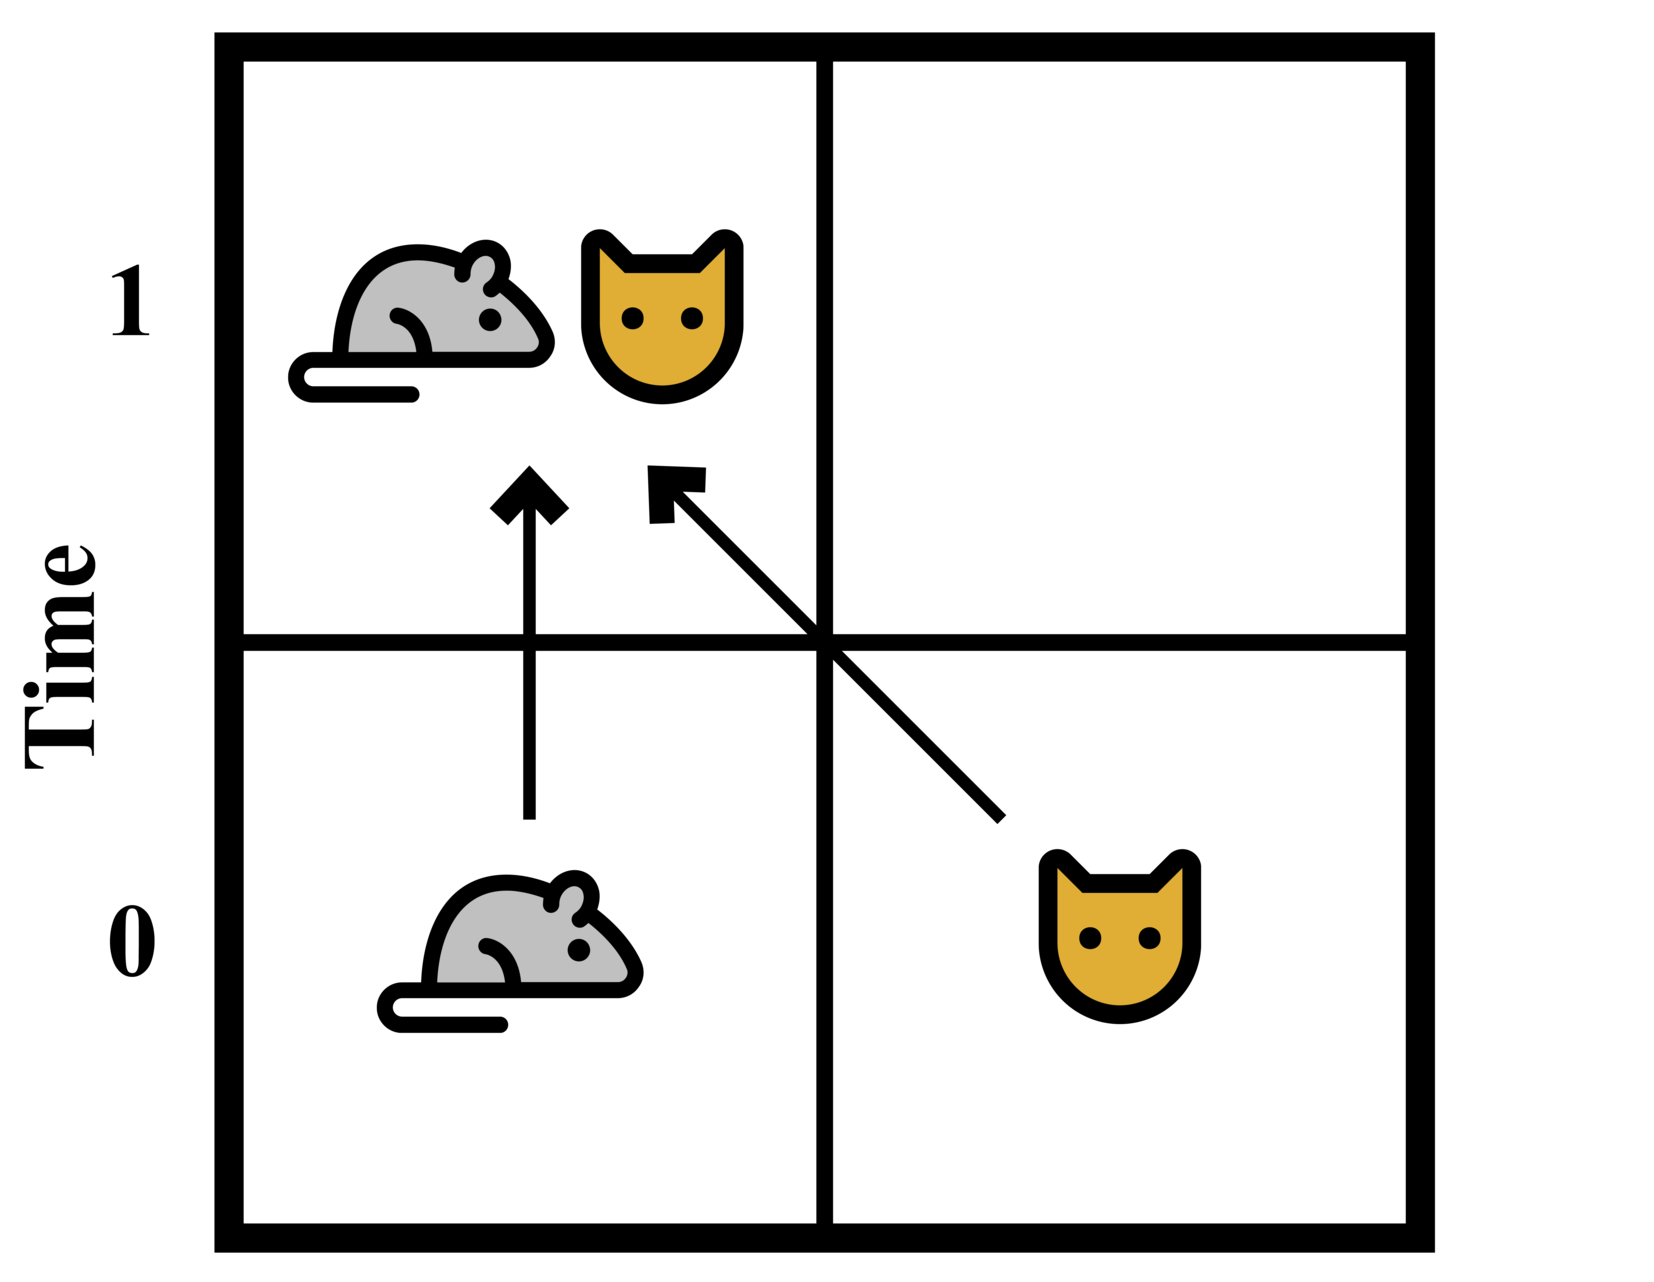
\includegraphics[scale=0.5]{figs/catMouseSm}
	}
	\caption{A simple cat and mouse model.\label{fig:AB-MCMC-1}}
\end{figure}


Let a model timestep be an array $E \in \mathbb{R}_{SA}$ whose elements $e_{\psi a}$ are the number of agents in state $\psi$ that perform act $a$ in this timestep. For example, the timestep shown in Figure~\ref{fig:AB-MCMC-1} for the cat and mouse example would be
\[
E = \kbordermatrix{
	& \alpha_0 & \alpha_1 \\
	\sigma_0 & 0 & 0 \\
	\sigma_1 & 1 & 0 \\
	\sigma_2 & 0  & 1 \\
	\sigma_3 & 0 & 0 \\
}
\]
where one agent in state $\sigma_1$ (\textit{right cat}) performs action $\alpha_0$ (\textit{move}) and one agent in state $\sigma_2$ (\textit{left mouse}) performs action $\alpha_1$ (\textit{stay still}).

Let a model trajectory, $T$, be an array in $\mathbb{R}^N_{SA}$ that represents $N$ timesteps of a model with $S$ agent states and $A$ actions, so that $T^t_{\psi a}$ denotes the $(\psi, a)^{th}$ element of the $t^{th}$ timestep matrix.

An array must satisfy a number of constraints in order to be a valid trajectory of an ABM. Since the elements of a trajectory are counts of agents, they must be non-negative integers. We'll call this the \textit{non-negative integer constraint} and define the set of all non-negative integer tensors
\begin{equation}
\mathbb{N}^N_{SA} = \left\{ T \in \mathbb{R^N_{SA}}: T^t_{\psi a} \ge \mathbf{0}^t_{\psi a}, T^t_{\psi a} \in \mathbb{Z}\right\}
\label{nonNegativeInt}
\end{equation}

A trajectory must also be \textit{continuous} by which we mean that the number of agents in each state at the end of timestep $t-1$ must be the number of agents in each state at the beginning of timestep $t$ plus the number of injections from the boundary conditions\footnote{This does not mean that agents cannot leave or enter the system, only that if they do then that change must be defined as part of an action.}. We call this the \textit{continuity constraint} and define the set of continuous arrays, with respect to an action function $F$:
\begin{equation}
\mathcal{C}^N_{SA}(F) = \left\{T\in\mathbb{R}^N_{SA}:  \forall \left(  1 \le \bar t < N\right): F^{\psi a}_{\phi} T^{t-1}_{\psi a} + I^t_\psi = \mathbf{1}^bT^{t}_{\phi b} \right\}
\label{continuous}
\end{equation}
where $F \in \mathbb{R}^{SA}_S$ is the action array $F^{\psi a}_* = F(\psi, a)$ and $I^t_\psi$ is the number of boundary condition injections into state $\psi$ at time $t$. Note that this assumes that a timestep is performed by updating all agents in parallel, i.e. agents must act with no information about the actions of other agents in the same timestep. This is different from serial update, where agents are updated in a particular order within a timestep and have access to information about the actions of agents that come before them in the ordering. Note also that this assumes that agents in the same state are indistinguishable, i.e. if we swap two agents in the same state, the trajectory is unchanged.


So, we define the set of trajectories, $\mathcal{T}^N_{SA}(F)$, as set of arrays that satisfy \eqref{nonNegativeInt} and \eqref{continuous}.
\begin{equation}
\mathcal{T}^N_{SA}(F) = \mathbb{N}^N_{SA} \cap \mathcal{C}^N_{SA}(F)
\label{SetOfTrajectories}
\end{equation}


\subsection{The posterior}

Our goal is to generate samples from the Bayesian posterior over the trajectories, boundary conditions and model parameters, given a set of observations, $\Omega$
\[
P\left(T,\theta \middle| \Omega\right) \propto P\left(\Omega \middle| T\right)P(T|\theta)P(\theta)
\]
$P(T|\theta)$, can be decomposed into the product of conditionals for each timestep and agent state
\[
P\left(T,\theta \middle| \Omega\right) \propto  P(\Psi^0|\theta) \prod_{t,\psi} P(T^t_{\psi *} | \Psi^t,\psi,\theta)
\]
where $\Psi^t\in\mathbb{R}_S$ is the model state at the start of timestep $t$ and $P(\Psi^0|\theta)$ comes from the boundary conditions in $\theta$\footnote{for notational clarity we assume that all injections are at time $t=0$, but this can easily be extended to injections at any timestep by adding $I^t_\psi$, as defined in equation \eqref{continuous}, to the model state along with $T$ and $\theta$ and replacing $P(\Psi^0|\theta)$ with $P(I^t_\psi|\theta)$.}.  The term $P(T^t_{\psi *} | \Psi^t,\psi,\theta)$ is the probability that $\Psi^t_\psi$ agents starting in state $\psi$ will collectively perform the vector of actions $T^t_{\psi *}$. The probability that a single agent performs action $a$ is given by the agent timestep $\pi_\theta(\psi,\Psi^t,a)$ (where we've added the subscript $\theta$ to emphasise its possible dependence on the parameters). Since agent actions are simultaneous, the collective behaviour is just the multinomial distribution given the individual agent timestep probabilities
\begin{equation}
P\left(T^t_{\psi *} \mid \Psi^t, \psi, \theta\right) = 
\begin{cases}
\Psi^t_\psi!\prod_a \frac{\pi(\psi,\Psi^t,a)^{T^t_{\psi a}}}{T^t_{\psi a}!} & \text{ if } T^t_{\psi a}\mathbf{1}^a = \Psi^t_\psi \\
0 & \text{otherwise}
\end{cases}
\end{equation}
If the trajectory is continuous then $\Psi^t = T^t_{* a}\mathbf{1}^a$ so 
\begin{equation}
P(T|\theta) =
\begin{cases}
P(\Psi^0 = T^0_{* c}\mathbf{1}^c|\theta)
\prod_{t, \psi} \left(T^t_{\psi b} \mathbf{1}^b \right)!
\prod_{a} \frac{\pi(\psi, T^{t}_{* d}\mathbf{1}^d,a)^{T^{t}_{\psi a}}}{T^{t}_{\psi a}!} & \text{if } T \in \mathcal{T}^N_{SA}(F) \\
0 & \text{otherwise}\\
\end{cases}
\label{priorTrajectory}
\end{equation}

The likelihood, $P(\Omega|T)$, can also usually be decomposed. Without loss of generality, we take $\Omega$ to consist of some number of observations that are independent of each other given the trajectory, so that $\Omega$ is a set of pairs $(\omega,v)$ that consist of a stochastic observation operator $\omega$ and an observed value $v$ (which may be a vector). We write $P(\omega(T)=v)$ to denote the probability of observation operator $\omega$ making observation $v$ on trajectory $T$. So
\[
P(\Omega|T) = \prod_{(\omega,v) \in \Omega} P(\omega(T)=v)
\]
and the posterior can be written in terms of the agent timestep function as
\begin{equation}
P(T,\theta|\Omega) \propto 
\begin{cases}
P(\theta)
P(\Psi^0 = T^0_{* c}\mathbf{1}^c|\theta)
\prod_{(\omega,v) \in \Omega}
P\left(\omega(T)=v\right)
\prod_{t, \psi} \left(T^t_{\psi b} \mathbf{1}^b \right)!
\prod_{a} \frac{\pi(\psi, T^{t}_{* d}\mathbf{1}^d,a)^{T^{t}_{\psi a}}}{T^{t}_{\psi a}!} & 
 \text{if } T \in \mathcal{T}^N_{SA}(F) \\
0 & \text{otherwise}\\
\end{cases}
\label{posterior}
\end{equation}

\section{Approximating the support of the posterior}\label{sec:approx_support}
%##########################################

As we saw in the introduction, sampling from equation \eqref{posterior} is difficult because it is hard to find proposal trajectories that have non-zero probability. Our strategy to solve this problem is to first derive an expression for a volume of trajectory/parameter space that bounds the support of the posterior, $\supp(P(T,\theta|\Omega))$ (i.e. the set of $\left<T,\theta\right>$ pairs that have non-zero posterior probability). If we choose a bounding volume that it is easy to sample from and is a relatively tight approximation of $\supp(P(T|\Omega)))$ then there's a good chance that a sample drawn from the volume will have non-zero probability. The bounding volume doesn't need to be exact, it just needs to tight enough to make it easier to find a non-zero probability sample.

From equation \eqref{posterior}
\begin{equation}
\begin{aligned}
\supp (P( T,\theta |\Omega)) = 
& \bigcap_{(\omega,v) \in \Omega,t, \psi, a} \mathcal{T}^N_{SA} \cap \supp(P(\theta)) \\ 
&\supp(P(\Psi^0 = T^0_{* c}\mathbf{1}^c)|\theta) \cap \\
& \supp\left(P\left(\omega(T)=v\right)\right) \cap \\
&\left( \supp\left(\pi_\theta(\psi,T^t_{* b}\mathbf{1}^b,a)\right) \cup \left\{T:T^t_{\psi a} = 0\right\} \right)
\end{aligned}
\label{support}
\end{equation}
i.e. in order for $\left<T,\theta\right>$ to have non-zero posterior probability, $\theta$ must have non-zero prior probability and $T$ must be a trajectory of the ABM that has a possible start state, all the observation likelihoods must be non-zero and each non-zero element of $T$ must denote an agent action with non-zero probability.

\subsection{Convex mixed-integer polyhedra}
%################################################################
\label{BPoly}

We'll now approximate the support in equation \ref{support} with a convex \textit{mixed-integer polyhedron}, $\mathcal{P}$, (see, for example, \citet{conforti2010polyhedral}) which we define to be a set of vectors, some of whose elements are integer and some real-valued, that satisfy a set of linear constraints:
\[
\mathcal{P} = \left\{ X\in\mathbb{Z}^N \times \mathbb{R}^M : L \le  CX \le U \right\}
\]
for some matrix $C$ and some vectors $L$ and $U$ .

Any linear inequality on $T$ and $\theta$ can be expressed in this form by letting $X$ consist of the elements of $T$ and $\theta$ flattened into one dimension so that
\[
X^i = W^{\psi a i}_{t}T^t_{\psi a} + G^i_j\theta^j
\]
and $W$ and $G$ have inverses
\[
\hat{W}^t_{\psi a i} = W^{\psi' a' i'}_{t'}\delta_{\psi'\psi}\delta_{a'a}\delta^{t't}\delta_{i'i}
\]
such that
\[
T^t_{\psi a} = \hat{W}^{t}_{\psi a i}X^i
\]
and
\[
\hat{G}^j_i = G^{i'}_{j'}\delta_{i'i}\delta^{j'j}
\]
such that
\[
\theta^j = \hat{G}^{j}_{i} X^i
\]
where $\delta^{ij}$ and $\delta_{ij}$ are 1 if $i=j$ and 0 otherwise. In this way we can switch unambiguously between $X$ and $\left<T,\theta\right>$.

From equation \ref{SetOfTrajectories} we can see immediately that the set of all trajectories, $\mathcal{T}^N_{SA}$, is is already defined as a set of linear constraints on $T$. The support of the prior $P(\theta)$ is usually of a simple form that can easily bounded, usually by a hyper-rectangle giving the range of each variable. The supports of the start state, $P(\Psi^0|\theta)$, the observations, $P(\omega(T)=v)$, and the agent actions, $\pi_\theta(\psi,T^t_{*b}\mathbf{1}^b,a)$, can often be easily expressed as linear constraints by hand. However, if this is not the case, each of the probability distributions can be expressed as computer programs. In practice, these computer programs will be simple and it will be possible to use a technique known as \textit{abstract interpretation} \citep{cousot1977abstract} using the domain of convex polyhedra \citep*{cousot1978automatic, becchi2018efficient, fukuda2020polyhedral} to efficiently calculate a convex polyhedron that bounds the support of the program. Software to perform abstract interpretation using convex polyhedra already exists \citep*{henry2012pagai, GN2021, jeannet2009apron, bagnara2008parma} and the technique has been used in applications such as compiler optimization \citep{nsjodin2009design} and verification of safety-critical systems \citep{halbwachs1997verification}. The programs may contain calls to a random number generator \texttt{Random()} that returns a random floating-point number $0 \le r < 1$. This can be represented in the polyhedral domain by introducing an real valued auxiliary variable, $r$, that satisfies $0 \le r < 1$ for each call to \texttt{Random()}. These auxiliary variables can be removed immediately using the abstract interpretation software to project the polyhedron back into the space of $X$. This relies on converting the polyhedron to its set of vertices \citep{motzkin1953double} and projecting the vertices, so the number of vertices must be of a tractable size. Alternatively, the auxiliary variables can be added to X and marginalised out when we take the samples.

If the number of agents is very much smaller than the number of agent states (which is often the case with agent based models) then we may be willing to make the assumption that in any timestep there is at most one agent performing a given action from a given start state (i.e. $\forall \psi, a, t: T^{\psi a}_t \in \{0,1\}$). Under this assumption, which we'll call the \textit{Fermionic assumption}, the set of \textit{Fermionic trajectories}, $\mathcal{F}^N_{SA} = \left\{T\in\mathcal{T}^N_{SA}: \forall \psi, a, t: T^{\psi a}_t \in \left\{0,1\right\}\right\}$, all lie on the corners of the unit hypercube. So the intersection of $\mathcal{F}^N_{SA}$ with any set is a convex polyhedron and $\supp(P(T|\Omega))$ can always be exactly represented as a mixed-integer polyhedron (although finding that polyhedron isn't always easy).

So, if we let $\mathcal{P}(f)$ be a mixed integer polyhedron that bounds $\supp(f)$ then from equation \eqref{support}
\begin{equation}
\begin{aligned}
\supp(P( T, \theta |\Omega)) \subseteq \mathcal{P}(P(T,\theta|\Omega)) =
& \bigcap_{(\omega,v) \in \Omega,t,\psi, a} \mathcal{T}^N_{SA} \cap \mathcal{P}(P(\theta)) \\
& \mathcal{P}(P(\Psi^0 = T^0_{* c}\mathbf{1}^c|\theta)) \cap\\
&    \mathcal{P}\left(P\left(\omega(T)=v\right)\right) \cap \\
& 
\left(\mathcal{P}\left(\pi_\theta(\psi,T^t_{* b}\mathbf{1}^b,a)\right)
\cup
\left\{T: T^t_{\psi a} = 0\right\}\right)
\\
\end{aligned}
\label{polyhedralSupport}
\end{equation}

The intersection of two mixed-integer polyhedra is easy to express as another mixed integer polyhedron by just concatenating the constraints
\begin{multline}
\left\{ X\in\mathbb{Z}^N \times \mathbb{R}^M : L \le  CX \le U \right\}
\cap
\left\{ X\in\mathbb{Z}^{N} \times \mathbb{R}^{M} : L' \le  C'X \le U' \right\}\\
= \left\{ X\in\mathbb{Z}^{N} \times \mathbb{R}^{M} : {L \choose L'}  \le   {C \choose C'}X \le {U \choose U'} \right\}
\label{intersection}
\end{multline}
so the only difficulty in calculating $\mathcal{P}(P(T,\theta|\Omega))$ from \eqref{polyhedralSupport} is the union in the final term. To transform this into an intersection we introduce an auxiliary variable $z$ and use the following identity: if the hyper-rectangle $0 \le X \le H$ bounds $L \le C X \le U$ for some vector $H \in \mathbb{Z}^N \times \mathbb{R}^M$, then for some given $i$ 
\begin{multline}
\left\{ X\in\mathbb{Z}^N \times \mathbb{R}^M : L \le C X \le U \right\}
\cup
\left\{X: X^i = 0, \mathbf{0} \le X \le H\right\}
= \left\{ \right.X\in\mathbb{Z}^N \times \mathbb{R}^M, z\in\{0,1\}:\\
CX + (\overline{B}-U)z \le \overline{B},\\
\underline{B} \le CX + (\underline{B}-L)z,\\
0 \le H^iz - X^i,\\
 z - X^i \le 0\\
\left. \right\}
\label{implication}
\end{multline}
where $\overline{B}$ are upper bounds on the values of $CX$ in the hyper-rectangle, defined as
\[
\overline{B} = \frac{\left(C+\left|C\right|\right)H}{2}
\]
where $|C|$ here denotes an element-wise absolute value of a matrix and $\underline{B}$ are lower bounds on the values of $CX$ defined as
\[
\underline{B}^i = \frac{\left(C - \left|C\right|\right)H}{2}
\]

To see why this identity holds, note first that the constraints make $z$ into an indicator variable that is 0 if $X^i=0$ or 1 otherwise. When $z=1$ the first constraint is equal to $CX \le U$ and the second is equal to $L \le CX$ so their intersection is $L \le  CX \le U$ as required, whereas when $z=0$ we have the constraints $\underline{B} \le CX \le \overline{B}$. But $\underline{B}$ and $\overline{B}$ are lower and upper bounds on the values of $CX$ in the hyper-rectangle so this is satisfied for all values $0 \le X \le H$ as required. 

There are two things worth noting here. Firstly if we make the Fermionic assumption then $z = T^t_{\psi a}$ and the auxiliary indicator variables become unnecessary. Secondly, we must bound $P(\pi_\theta(\psi,T^t_{*b}\mathbf{1}^b,a))$ by a hyper-rectangle with its lower corner at the origin. In practice, this is not a problem as we can just make a change of variable, shifting any variables that don't have zero as lower bound and multiplying by -1 if necessary, and give an upper bound such that the probability of any $\left<T,\theta\right>$ of interest having any element larger than $H$ is small.

So, by using \eqref{polyhedralSupport}, \eqref{intersection} and \eqref{implication} the support of the posterior can be reduced to a mixed-integer polyhedron.

As a simple illustration, consider a two-timestep trajectory of the cat and mouse model described in section \ref{abmdef}. Suppose we flip a fair coin to decide whether each agent state is occupied or empty at $t=0$. Suppose also that we observe a cat in the left grid-square at time $t=1$. We won't introduce any parameters so our aim is to construct a mixed-integer polyhedron that describes the support of the posterior $P(T|\Omega)$.

Working through \eqref{polyhedralSupport} term by term, the $\mathcal{T}^2_{4\,2}$ term is just the non-negative integer constraints and continuity constraints in \eqref{nonNegativeInt} and \eqref{continuous}, which are already in linear form so we're done. The second term is the support of the prior over the parameters which we ignore since there are no parameters. The next term is the support of the start state, this constrains each agent state at $t=0$ to be at most 1, which can be expressed as
\[
\left\{T:T^0_{\psi 0} + T^0_{\psi 1} \le \mathbf{1}_{\psi}\right\}
\]

The fourth term is the support of the observation. Since we observe a cat in the left grid-square at time $t=1$ we need to add the constraint
\[
T^1_{0 0} + T^1_{0 1} = 1
\]
The final term is the constraint due to agent interactions. The impossible interactions are a mouse staying put when there is a cat on the same gridsquare or moving when there are no cats, so we constrain against these
\begin{equation}
\begin{aligned}
\supp(\pi(2,T^t_{* a}\mathbf{1}^a,0)) &= \left\{ T: -T^t_{0 0} - T^t_{0 1} \le -1 \right\}\\
\supp(\pi(3,T^t_{* a}\mathbf{1}^a,0)) &= \left\{ T: -T^t_{1 0} - T^t_{1 1} \le -1 \right\}\\
\supp(\pi(2,T^t_{* a}\mathbf{1}^a,1)) &= \left\{ T: T^t_{0 0} + T^t_{0 1} \le 0 \right\}\\
\supp(\pi(3,T^t_{* a}\mathbf{1}^a,1)) &= \left\{ T: T^t_{1 0} + T^t_{1 1} \le 0 \right\}
\end{aligned}
\label{actionConstraints}
\end{equation}
for all t. If, for simplicity, we make the Fermionic assumption by adding the constraints
\[
\mathbf{0}^t_{\psi a} \le T^t_{\psi a} \le \mathbf{1}^t_{\psi a}
\]
then using the identity in \eqref{implication} to take the union of each constraint in \eqref{actionConstraints} with $\left\{T: T^t_{\psi a} = 0, \mathbf{0} \le T \le \mathbf{1}\right\}$ finally gives the four constraints
\[
\begin{aligned}
-T^t_{0 0} - T^t_{0 1} + T^t_{2 0} & \le 0\\
-T^t_{1 0} - T^t_{1 1} + T^t_{3 0} & \le 0\\
T^t_{0 0} + T^t_{0 1} + 2T^t_{2 1} & \le 2 \\
T^t_{1 0} + T^t_{1 1} + 2T^t_{3 1} & \le 2
\end{aligned}
\]
for each timestep $t=0$ and $t=1$.

Taken together, these constraints define a polyhedron that bounds the set of (Fermionic) trajectories for the cat and mouse ABM.

\section{Sampling from the posterior}\label{sec:posterior_sampling}
%#################################################

Having shown how to approximate $\supp(P(T,\theta|\Omega))$ as a mixed-integer polyhedron, we now need to devise a way to use this to sample from $P(T,\theta|\Omega)$.

\citet{baumert2009discrete} presents a very general algorithm for sampling from any weighted subset of integer points within a bounding hyper-rectangle. The algorithm relies on sampling points on a random walk. However, in our case the number of valid trajectories is a vanishingly small proportion of the number of integer points in the smallest bounding hyper-rectangle, so a random walk is unlikely to come across any valid trajectories. Universal hashing \citep{meel2016constrained} provides a promising alternative but we have found that this technique doesn't scale to the number of dimensions needed for our application.

The Metropolis-Hastings algorithm is another well known and widely used sampling algorithm and this is the approach we use here. To do this we need to define
\begin{itemize}
\item a set of Markov states, $\mathcal{M}$

\item a probability distribution $P: \mathcal{M} \to \mathbb{R}$ which gives the probability of each Markov state (this need not be normalised as the Metropolis Hastings algorithm only ever needs probability ratios)

\item a stochastic proposal function $f:\mathcal{M} \to \mathcal{M}$ from which we can generate proposal transitions from one Markov state to another

\item a mapping $E:\mathcal{M} \to \mathbb{R}^T_{SA} \times \mathbb{T}$ which maps Markov states to trajectories and parameter values so we can recover the sample.
\end{itemize}

In order to be of use in practice, the proposal function, $f$, must have the following properties:
\begin{itemize}
	\item For any two Markov states there should exist a sequence of transitions which forms a path between those states and has non-zero probability of being proposed.
	
	\item For any proposal from state $S_a \to S_b$ with non-zero probability, the probability of the reverse transition from $S_b \to S_a$ should also be non-zero. This allows us to attain detailed balance in the Metropolis Hastings algorithm. The average ratio of forward and backward probabilities times the ratio of start and end state probabilities should be close to 1 to ensure that a reasonable proportion of proposals are accepted.
	
	\item Given a current Markov state, there should be computationally efficient procedure to generate a proposal and calculate its acceptance probability. 
\end{itemize}

\subsection{The set of Markov states}
%#############################################

Given a polyhedron, we split the constraints into two sets: equalities (i.e. those whose lower and upper bound have the same value) and inequalities (i.e. those whose lower and upper bounds differ):
\begin{equation}
\mathcal{P} = \left\{X \in \mathbb{Z}^N \times \mathbb{R}^M: \left(L \le CX \le U\right) \cap \left(DX = E\right) \right\}
\label{zPolySupport}
\end{equation}

Our aim will be to use the equality constraints to reduce the dimension of the problem.

Suppose there are $N_e$ equality constraints (i.e. $E$ is an $N_e$ dimensional vector) and we partition the elements of $X$ into `basic' and `non-basic' elements, $X_B$ and $X_N$ respectively, so that there are exactly $N_e$ basic elements and $|X| - N_e$ non-basic elements (note that since the continuity constraints \eqref{continuous} are equality constraints then $N_e \ge (N-1)S$ ).

If we let $Q$ be a permutation matrix that separates the basic from non-basic elements so that
\[
QX = {X_B \choose X_N}
\]
then we can write
\[
DX = DQ^{-1}{X_B \choose X_N} = \left(B \mid N\right){X_B \choose X_N} = E
\]
so
\begin{equation}
BX_B + NX_N = E
\label{eqconstraints}
\end{equation}

Now, since there are $N_e$ basic variables and $N_e$ equality constraints, $B$ is square so if we choose the basic variables in such a way as to ensure that $B$ has an inverse then
\begin{equation}
X_B = B^{-1}(E - NX_N)
\label{basicvars}
\end{equation}
so letting
\[
V = Q^{-1}{B^{-1}E \choose \mathbf{0}}, \, M = Q^{-1}{-B^{-1}N \choose \mathbf{1}}
\]
\begin{equation}
X = V + MX_N
\label{markovtotrajectory}
\end{equation}
In section \ref{basis} we'll show how to choose $X_B$ to ensure that $B$ has an inverse and the integer dimensions of $X_B$ remain integer as long as the integer dimensions of $X_N$ are integer. Given this, then the original polyhedron is equivalent to the reduced dimension polyhedron
\begin{equation}
\mathcal{P}' = \left\{X_N \in \mathbb{Z}^{N'} \times \mathbb{R}^{M'}: L-CV \le  CMX_N \le U-CV\right\}
\label{reducedPolySupport}
\end{equation}
where $N'$ and $M'$ are the number of integer and real-valued elements remaining in $X_N$.

Since $Q$ is just a permutation matrix, $X_N$ and $X_B$ can be bound within hyper-rectangles by transforming the $\mathcal{P}$-bounding hyper-rectangle, $H$, from section \ref{BPoly}
\[
QH = {H_B \choose H_N}
\]
So, $X_N$ is bound by $0 \le X_N \le H_N$. Given this, we define the set of Markov states to be
\[
\mathcal{M} = \left\{ X_N: 0 \le X_N \le H_N \right\}
\]
where each Markov state, $X_N$, is mapped to a unique trajectory, $X$, using \eqref{markovtotrajectory}.

\subsection{The probability of a Markov state}

Given a Markov state, $X_N$, that satisfies $0 \le X_N \le H_N$, the associated trajectory given by equation \eqref{markovtotrajectory} is guaranteed to satisfy all the equality constraints. However, there is no guarantee that the basic variables given by eq \eqref{basicvars} will be within their bounds $0 \le X_B \le H_B$ or that the constraints $L \le CX \le U$ will be satisfied. To deal with this we introduce the concept of \textit{infeasibility} which is a measure of the extent to which a Markov state fails to satisfy these constraints.

Let the infeasibility function $\iota(l,x,u)$ be defined to be equal to 0 if $l < x < u$ or equal to the distance to the nearest bound otherwise
\[
\iota(l,x,u) =
\begin{cases}
x-u & \text{if }x>u\\
l-x & \text{if }x<l\\
0 & \text{otherwise}
\end{cases}
\]
extend this concept to vectors by summing the infeasibility of each element so
\[
\iota(L,X,U) = \sum_i \iota(L_i,X_i,U_i)
\]
now define the infeasibility of a model state, $X$, be the sum of infeasibilities of all constraints
\[
\iota(X) = \iota(L, CX, U) + \iota(0, X, H)
\]
this implies that a Markov state has an infeasibility of $\iota(V + MX_N)$. If this infeasibility is zero, then all the constraints are satisfied and the (unnormalised) probability of the Markov state is defined to be equal to the joint probability, which is proportional to the posterior
\[
P(X_N) = P(X=V + MX_N,\Omega) = P(T,\theta|\Omega)P(\Omega)
\]

If the infeasibility is not zero, then the probability is defined in the following way. First define the \textit{clamp} function
\[
c(l,x,u) \begin{cases}
l & \text{if }x<l\\
u & \text{if }x>u\\
x & \text{otherwise}
\end{cases}
\]
and a \textit{clamped} trajectory
\[
\overline{\underline{X}} = \sum_i c(0,X_i,H_i)
\]

Next we introduce a function that is approximately equal to $P(T,\theta,\Omega)$ inside the polyhedron, but is also well defined and non-zero inside the whole hyper-rectangle $H$. We define the approximation as decomposable into functions on each individual agent act $T^t_{\psi a}$
\[
g(T,\theta) = \prod_{t,\psi,a} g^t_{\psi a}(T^t_{\psi a},\theta) \approx P(T,\Omega|\theta)P(\theta) = P(T,\theta,\Omega) \text{ if }\left<T,\theta\right>\text{ is feasible}
\]
Now let $R$ be a function that is 1 inside a hyper-rectangle $L \le X \le U$ and decays exponentially outside
\[
R(L,X,U) = e^{\frac{-\iota(L,X,U)}{\tau}}
\]
where $\tau$ is a tunable parameter that controls the rate of exponential decay.

We now define an augmented function that combines these functions
\begin{equation}
g_a(X,A) = R\left(L,A,U\right)R(0,X,H)g\left(\hat{F}^t_{\psi a i}\overline{\underline{X}}^i, \hat{G}^j_i\overline{\underline{X}}^i\right)
\label{augmentedG}
\end{equation}
so that we can define a function that approximates $P(X,\Omega)$ within the feasible region of $X$ and is exponentially attenuated outside that region, so 
\[
g(X) = g_a\left(X,CX\right) \approx P(T,\theta,|\Omega)
\]

For infeasible trajectories, we define the probability, $P_\iota$, to be
\begin{equation}
P_\iota(X_N) \propto g(V+MX_N)
\label{loglinprob}
\end{equation}

This means that infeasible states have non-zero probability and the Markov chain will pass through some infeasible states.  However, if we just ignore these and only take samples from feasible states then we end up with samples from the true posterior. Allowing the Markov chain to pass through infeasible states has the advantage of ensuring that there exists a path between any two feasible states and improves mixing. When used in the context of a particle filter, it also solves the problem of unexpected observations that can't be generated by any particle, as we can allow the particles to become temporarily infeasible. The price we pay for this is the computational cost of moving through infeasible states that don't generate useful samples.

The approximating functions $g^t_{\psi a}$ do not affect the stationary state of the Markov chain in the feasible region so can be any arbitrary function that is non-zero inside the hyper-rectangle. However, we'll see in the next section that a proposal is more likely to be accepted if the approximation is better, so a better approximation leads to a more efficient algorithm. We have found that approximating $g^t_{\psi a}$ as 
\[
g^t_{\psi a}(T^t_{\psi a},\theta) = \int P(T^t_{\psi a}|\theta')P(\theta')d\theta' \prod_{\left<\omega,v\right> \in \Omega} \int P(\omega(T)=v|T)P(T|\theta'')P(\theta'') dT  d\theta''
\]
gives acceptable performance. Note that the the product term is constant for all $g^t_{\psi a}$ and the $\theta$ dependence of $g^t_{\psi a}$ has been marginalised out; there may be model-specific ways of retaining some $\theta$ dependence as appropriate. The first integral can easily be found by sampling from the prior (i.e. drawing from $P(\theta)$  then drawing from $P(\Psi^0|\theta)$, then executing the model) and marginalising for each $t$, $\psi$ and $a$. Each of the integrals in the product term can also be approximated using the same samples from the prior.

If we define the \textit{energy} of a Markov state to be
\[
E(X_N) =
\begin{cases}
-\tau log(P(X_N)) & \text{if }  \iota(Y) = 0\\
-\tau log(P_\iota(X_N)) & \text{otherwise}
\end{cases}
\]
then the probability of a Markov state can be written in the form
\begin{equation}
P(Y) \propto e^{\frac{-E(X_N)}{\tau}}
\end{equation}
This is a Boltzmann distribution which describes a thermodynamic system at equilibrium with a heat bath of ``temperature'' $\tau$. It has been shown that simulations of thermodynamic systems of this type are able to solve large integer optimisation problems which are similar in structure to the one here \citep{kirkpatrick1983optimization}. In our case, we don't need to change the temperature during the sampling process, but we do need to choose a value for $\tau$. Higher temperatures will increase mixing in the Markov chain, but will also increase the proportion of time spent in infeasible states so we need to find a temperature that is high enough to ensure good mixing of the chain but low enough to ensure a reasonable proportion of samples are feasible. We have found that a good rule of thumb is to set the temperature so that 50\% of the samples in a chain are infeasible.

\subsection{Transitions between Markov states}

Transitions between states always either perturb the trajectory or the parameters, never both. Trajectory perturbations change a single trajectory-element of $X_N$ by $\pm 1$. If the element is already on one of its bounds on the hyper-rectangle, $H_N$, it is only ever perturbed in the feasible direction. So, the set of trajectory perturbations from state $X_N$ is given by
\[
\mathcal{D}(X_N) = \left\{X'_N : X'_N = X_N + \delta e_i, 0 \le X'_N \le H_N, \delta \in \left\{+1,-1\right\}, i \in \mathcal{V} \right\}
\]
where $e_i$ is the unit vector with a 1 in the $i^{th}$ element and $\mathcal{V}$ is the set of indices of $X_N$ that correspond to elements of the trajectory.

The most appropriate set of parameter perturbations is highly model specific so it's difficult to give a universally applicable scheme. However, in the absence of any model-specific schemes, one very general way to do this is to consider only single-parameter perturbations. Integer parameters can be perturbed in the same way as trajectory perturbations, real-valued parameters can be perturbed by a Gaussian whose mean is 0 and whose standard deviation is some fraction of the range of the parameter in $H_N$. Any probability mass that falls outside of $H$ is interpreted as a transition back to the original state.

\subsubsection{The the probability of proposals}

Given a Markov state, we choose a transition to another state by first choosing, with fixed probability, whether to perturb the trajectory or the parameters. This allows us to control the speed at which the trajectory changes compared to the parameters, it's likely that we'll want to update the trajectory more often than the parameters.

For trajectory perturbations, given a current state $X_N$, associate a probability with each proposed state $X'_N \in \mathcal{D}(X_N)$
\begin{equation}
P(X_N \to X'_N) = \frac{\min\left(1, \frac{P_\iota(X'_N)}{P_\iota(X_N)}\right)}{S(X_N)} 
\label{transitionProb}
\end{equation}
where $P_\iota$ is the probability defined in \eqref{loglinprob} and
\begin{equation}
S(X_N) = \sum_{X'_N \in \mathcal{D}(X_N)} \min\left(1, \frac{P_\iota(X'_N)}{P_\iota(X_N)}\right)
\label{transitionSum}
\end{equation}
In the next section we'll see how to calculate this value efficiently.

In order to choose a transition, we draw a destination state $X'_N \in \mathcal{D}(X_N)$ with probability $P(X_N \to X'_N)$. The Metropolis-Hastings acceptance probability is then
\[
\alpha = 
\min\left( 1, \frac{P(X'_N)P(X'_N \to X_N)}{P(X_N)P(X_N \to X'_N)} \right) = \min\left(1, 
\frac{P_\iota(X_N)}{P(X_N)} \frac{P(X'_N)}{P_\iota(X'_N)}  \frac{S(X_N)}{S(X'_N)}\right)
\]
When $X_N$ is infeasible $\frac{P_\iota(X_N)}{P(X_N)} = 1$. When $X_N$ is feasible $P_\iota(X_N)$ approximates $P(X_N)$ so their ratio should be close to 1. Similarly for $X'_N$. Finally, we'll see in the next section that if we choose the basis carefully then $S(X_N)$ will not change very much between transitions so the ratio $ \frac{S(X_N)}{S(X'_N)}$ should also be close to 1 meaning that the acceptance probability should also be close to 1.

\subsection{Choosing a basis}
\label{basis}
The definition of the Markov chain depends on a partition of the model state into basic and non-basic variables such that $B$ in equation \eqref{basicvars} has an inverse, $B^{-1}$, and if $X_N \in \mathbb{Z}^{N'} \times \mathbb{R}^{M'}$ then $X \in \mathbb{Z}^{N} \times \mathbb{R}^{M}$ (i.e. if $X_N$ has all integers in the correct elements then so does $X$). In general there exist many partitions that satisfy these requirements so it remains to define a method of choosing one. The choice of basis affects the efficiency of trajectory transitions via:
\begin{itemize}
\item the computational cost of recomputing $S(X_N)$

\item the probability that the proposal is accepted via the ratio of sums $S(X_N)/S(X'_N)$

\item the mixing rate of the Markov chain, since the choice of basis affects the way the probability distribution in $X$ space is projected into $X_N$ space.
\end{itemize}

Taking each in turn, $S(X_N)$ depends only on ratios of $P_\iota$. However, if we project $S(X_N)$ into the augmented state space $X_a = {X \choose CX} = {I \choose C}(V + MX_N)$ of $g_a$ (equation \eqref{augmentedG}) then the $P_\iota$s can be expressed as a product of functions on elements of $X_a$. So, when recalculating the sum in equation \eqref{transitionSum} after a transition from $X_N$ to $X_N + \delta e_i$, the only terms that change are those from $X_N + \delta e_j \in \mathbb{D}(X_N)$ such that the non-zero elements of ${I \choose C}(\delta Me_j)$ intersect with the non-zero elements of ${I \choose C}(\delta Me_i)$. So, if we choose a basis such that ${M \choose CM}$ is sparse then re-calculation of $S(X_N)$ will only require a few terms to be recalculated and so will be more efficient. A binary tree data structure can be used to efficiently update and draw from the probability distribution over transitions in equation \eqref{transitionProb} while also keeping track of $S(X_N)$ \citep{TangMutableCategorical}.

This same idea extends to the ratio $\frac{S(X_N)}{S(X'_N)}$. If ${M \choose CM}$ is sparse, and also short, then we should expect the ratio of sums to be close to 1.

The Markov chain will also mix better if the columns of ${M \choose CM}$ are short. \citet{mihelich2018maximum} shows that the Kolmogorov-Sinai entropy of the Markov process is a good proxy for its mixing speed. In the context of our algorithm the entropy is higher if the neighbours of a Markov state have similar probability, all else being equal. If ${M \choose CM}$ is sparse and short then we expect the probability of adjecent Markov states to be similar.

[TODO: Finding a short basis is lattice reduction, which is hard?]

In order to find a sparse basis that maintains the integer elements, we use the following algorithm. Starting with a mixed-integer polyhedron expressed in the form
\[
\mathcal{P} = \left\{X \in \mathbb{Z}^N \times \mathbb{R}^M: L \le CX \le U \cap DX = E \right\}
\]
If we let
\[
W= {D \choose C}
\]
and
\[
F = {E \choose \mathbf{0}}
\]
then
\begin{equation}
\mathcal{P} = \left\{X \in \mathbb{Z}^N \times \mathbb{R}^M: {\mathbf{0} \choose L} \le W X - F \le {\mathbf{0} \choose U} \right\}
\label{jointconstraints}
\end{equation}

Our aim is to mark variables from $X$ as basic one at a time. Once we're done, the remaining variables will make up the non-basic variables, $X_N$.

Given a set of constraints in the form \eqref{jointconstraints}, we mark the $j^{th}$ element of $X$ as basic and the $i^{th}$ equality constraint as ``reduced'' by choosing an element $W^i_j$ to be a \textit{pivot point} and performing Gaussian elimination on the $j^{th}$ column of $W$ so that $W^i_j$ is the only non-zero element in the column $W_j$. So
\[
{\mathbf{0} \choose L} \le GWX - GF \le {\mathbf{0} \choose U}
\]
where $G$ is the matrix
\[
G =  
\begin{pmatrix}
1 &  & &-\frac{W^0_j}{W^i_j} & & &\\
& \ddots & &\vdots & & &\\
& & 1 & -\frac{W^{i-1}_j}{W^i_j} & & &\\
& & & \frac{1}{W^i_j} & & &\\
& &  & -\frac{W^{i+1}_j}{W^i_j} & 1 & &\\
& & & \vdots & & \ddots &\\
& & & -\frac{W^n_j}{W^i_j} & & &1\\
\end{pmatrix}
\]

Letting $\hat{W} = GW$ and $\hat{F} = GF$ recovers the canonical form
\begin{equation}
{\mathbf{0} \choose L} \le \hat{W}X - \hat{F} \le {\mathbf{0} \choose U}
\label{eliminatedConstraint}
\end{equation}
but now with the $j^{th}$ element of $X$ marked as basic and the $i^{th}$ row of $\hat{W}$ marked as ``reduced''. We now repeat the process until no more equality constraints can be reduced.

The use of Gaussian elimination here ensures that $B^{-1}$ exists. In order to ensure that $X_B$ has the correct integer structure, given that $X_N$ does, we add the requirement that we can only mark integer elements of $X$ as basic on a pivot point $W^i_j$ such that the row vector $W^i$ is zero on all non-integer columns and $W^i_j$ divides $W^i_k$ for all $k$ (so for rows that have a non-zero element on a real-valued column, we always eliminate on a real-valued column). This constraint ensures that a reduced equality constraint has the form $X_B^i = F_i - W^iX_N$ where $W^i$ is a row vector of integer coefficients on integer elements of $X_N$. If this constraint has any all-integer solution then $F$ must also be an integer. So, if $X_N$ has the correct integer structure, then $X_B^i$ is also an integer. Note that, even with this constraint, we can always eliminate all continuity constraints.

This defines a set of valid pivot points at each elimination step. In order to decide which point to choose, we note that when we pivot on $W^i_j$, $GW$ differs from $W$ in at most 
\[
\mu = (\left|W_j\right|_0-1)(\left|W^i\right|_0-1)
\]
 elements, where $\left|\cdot\right|_0$ is the L0-norm (i.e. the number of non-zero elements in a vector or matrix). So, this gives an upper bound on $\left|WG\right|_0 - \left|G\right|_0$, the change in L0-norm (or reduction in sparsity) of $W$ when we pivot on $W^i_j$. It has been found that choosing $W^i_j$ to be the element that minimises $\mu$ (known as the Markowitz criterion) is a computationally efficient way of maintaining the sparsity of a matrix while performing Gaussian elimination \citep*{markowitz1957elimination, suhl1990computing, maros2002computational}. So, in order to find a sparse basis, we calculate the set of valid pivot points, choose the point that minimises $\mu$, perform the pivot and repeat until no more valid pivot points remain. \citet{suhl1990computing} shows how to perform this in a computationally efficient way.

\section{Spatial predator-prey demonstration}\label{sec:demonstration}

We demonstrate the above techniques on a 32x32 grid of ``predator'' and ``prey'' agents. At each timestep a prey agent either moves to an adjacent grid-square (i.e. up, down, left or right with equal probability), dies or gives birth to another prey agent on the an adjacent grid-square. Predators also either move to an adjacent grid-square, die or give birth. However, predators only give birth when there is at least one prey on an adjacent grid-square. In addition, if a prey has any predators on adjacent grid-squares there is a chance it may be eaten. The probability of each behaviour is shown in table \ref{rates}.

\begin{table}
	\begin{center}
		\begin{tabular}{llllc}
		\hline
		Aget type & Adjacent agents & Behaviour & Probability\\
		\hline
		Prey & No predators & die &        0.100\\
			& & give birth &        0.156\\
			& & move &        0.744\\
			& &&\\
		Prey & Predators > 0 & die &        0.100\\
			& & give birth &        0.156\\
			& & be eaten &        0.300\\
			& & move &        0.444\\
			& &&\\
		Predator  & No prey & die  &      0.100\\
			& & move &        0.900\\
			& &&\\
		Predator  & Prey > 0 & die  &      0.100\\
			& & give birth &        0.300\\
			& & move &        0.600\\
		\hline& 
		\end{tabular}
	\end{center}
	\caption{The probabilities of each behaviour in the predator-prey model}
	\label{rates}
\end{table}

\begin{figure}
	\centering
	\resizebox{0.5\textwidth}{!}{
		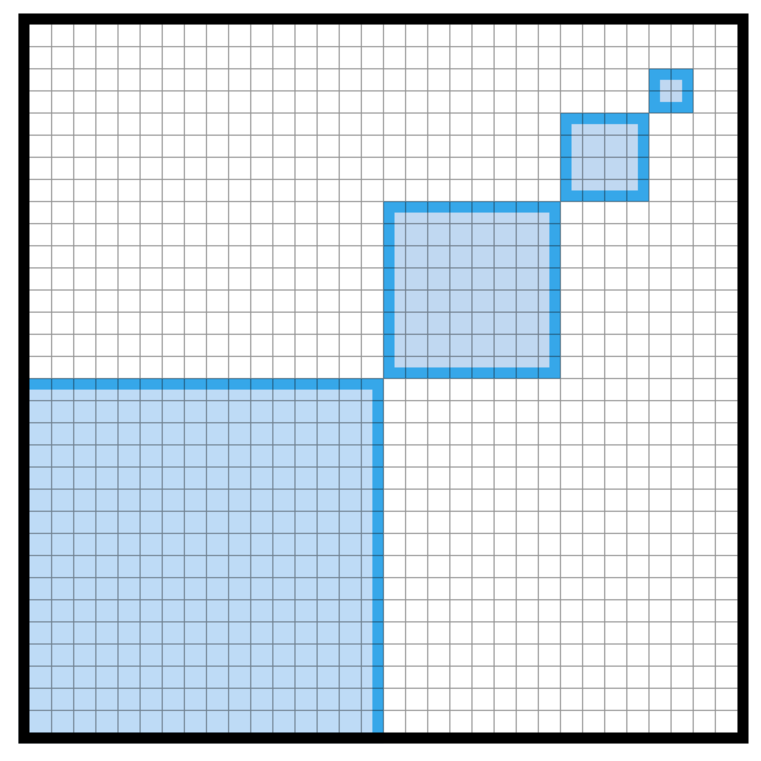
\includegraphics[scale=0.5]{figs/gridRegionsSm.png}
	}
	\caption{Summary statistics consist of the total number of agents in each of the four shaded regions.}
	\label{figRegions}
\end{figure}

\begin{figure}
	\centering
	\resizebox{0.8\textwidth}{!}{
		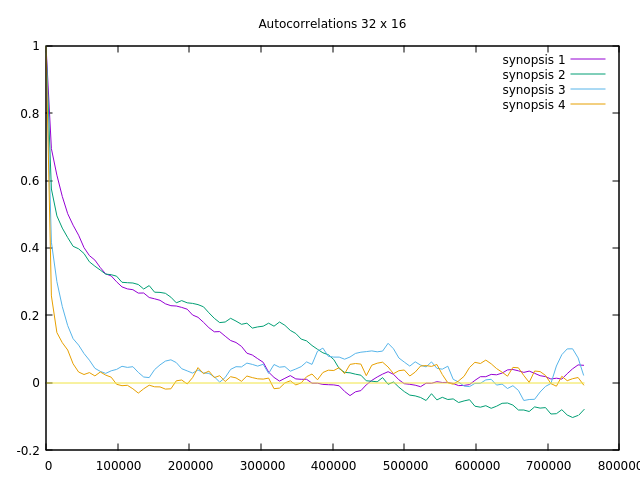
\includegraphics{figs/PredPrey32-16-graph.png}
	}
	\caption{Mean autocorrelation for each scalar of the summary statistics, averaged over all chains.}
	\label{figAutocorrelation}
\end{figure}

\begin{figure}
	\centering
	\resizebox{0.8\textwidth}{!}{
		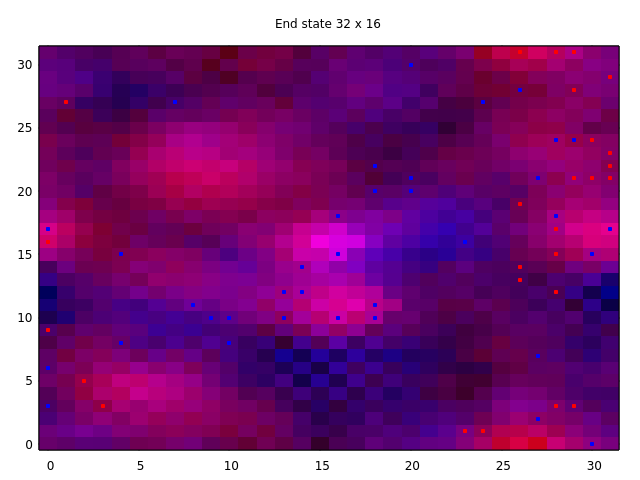
\includegraphics{figs/PredPrey32-16-map.png}
	}
	\caption{Mean number of agents in each gridsquare after the last timestep, averaged over all samples. Blue represents predator, red represents prey. The dots represent the final positions of agents in the simulation from which the observations were generated. The background colour of each square has red/blue intensity proportional to the log of the mean number of prey/predators in that square, respectively.}
	\label{figEndState}
\end{figure}


Simulated observation data was generated by performing a forward simulation of the model. The number of predators and prey in each gridsquare at the start of the simulation was drawn from a Poisson distribution with rate parameter $\lambda = 0.05$. The model was then simulated forward for 16 timesteps. At each timestep, each gridsquare was observed with a probability of 0.02. If an observation was made, the number of predators in the gridsquare was observed. In order to demonstrate assimilation with observational noise, each predator was observed with probability 0.9 (i.e. the number observed was drawn from a Binomial distribution. Note that our algorithm can also assimilate observations with no noise). The same procedure was then repeated for prey.

Four separate Markov chains of 1,500,000 samples each were generated from the posterior using the method described above. The start state for each chain was drawn from the prior (i.e. model trajectory without any observations). The first 200,000 samples of each chain were discarded and the remaining samples were split into first and last halves to give 8 sample sequences in total. 

In order to assess the convergence of the chains, a set of summary statistics were calculated for each sample of each chain. The summary statistics consisted of the total number of agents within the shaded regions shown in figure \ref{figRegions} measured at the end of the last timestep of the trajectory. This arrangement of regions was chosen in order to capture the convergence at different spatial scales. From the summary statistics, we calculated the the Gelman-Rubin diagnostic \cite{gelman1992inference}, and approximated the autocorrelation at various time lags. Using the notation $x_{ij}$ to refer to a scalar statistic of the $i^{th}$ sample of the $j^{th}$ sequence, given $m$ sequences of $n$ samples each, let $\bar{x}_j$ be the mean of the $j^{th}$ sequence and $\bar{x}$ be the mean over all sequences
\[
\bar{x}_j = \frac{1}{n}\sum_{i=1}^n x_{ij}, \bar{x} = \frac{1}{m}\sum_{j=1}^m \bar{x}_j
\]
let $W$ be the within-sequence variance
\[
W = \frac{1}{m} \sum_{j=1}^m \frac{1}{n-1} \sum_{i=1}^n (x_{ij} - \bar{x}_j)^2
\]
and $B$ be the between-sequence variance
\[
B = \frac{n}{m-1}\sum_{j=1}^m (\bar{x}_j - \bar{x})^2
\]
Following\cite{gelman2013bayesian}, an overapproximation of the true variance of the statistic can be calculated as
\[
\widehat{\text{var}}^+ = \frac{n-1}{n}W + \frac{1}{n}B
\]
and the Gelman-Rubin statistic can be defined as
\[
\hat{R} = \sqrt{\frac{\widehat{\text{var}}^+}{W}}
\]
This gives a measure of the uncertainty in the standard deviation of the statistic due to the fact that we have only taken a finite number of samples. If this number is close to 1, then we have some justification in believing that we have taken enough samples.

[TODO: what was R?]

Also following\cite{gelman2013bayesian}, we approximated the autocorrelation as
\[
\hat{\rho}_t = 1 - \frac{V_t}{2\widehat{\text{var}}^+}
\]
where
\[
V_t = \frac{1}{n-t} \sum_{i=1}^{n-t} (x_i - x_{i+t})^2
\]

Figure \ref{figAutocorrelation} shows $\hat{\rho}_t$ as a function of $t$ for each scalar in the summary statistics. A decline of $\hat{\rho}_t$ to zero long before $t$ reaches the total number of samples, shows good convergence of the chain. The rate of this decline can be used to calculate the effective number of samples, defined as
\[
\hat{n}_e = \frac{mn}{1 + 2\sum_{t} \hat{\rho}_t}
\]
where the sum runs until $\hat{\rho}_t \le 0$. This approximates of the number of samples from a perfect IID sampler that would give the same uncertainty in the mean of the statistic.

[TODO: what was the effective sample size?]

Finally, figure \ref{figEndState} shows the mean number of agents at the end of the simulation, averaged over all samples. This is a visual way of showing that the observations have given rise to a posterior that gives some information about the true positions of the agents.

[Show convergence with problem size/number of constraints or with grid-size / number of timesteps (number of agents?)]

\section{Discussion} 
\label{discussion}

 
\subsection{Integration into sequential MCMC}

If we would like to perform online data assimilation or assimilation over a long time period, the above algorithm can be used as part of a sequential MCMC algorithm.

The \textit{Resample-Move} algorithm presented in \citet{gilks2001following} adds MCMC transitions to sequential importance resampling by adding a \textit{move} step after the resample step. At each move step each sample, $T^i_t = \left<\tau_{1:t}^i,\theta\right>$, is ``moved'' by initialising the Markov chain with $T^i_t$ and drawing a single new sample $T'^{i}_{t} \sim P(T_t|\Omega_{1:t})$. This solves the problem of particle impoverishment because even if multiple samples collapse to the same state during the resample step, the subsequent move step is likely to move them apart again. The algorithm remains exact because the samples coming out of the $m^{th}$ resample step are already distributed according to the target distribution, $P(T_t|\Omega_{1:t})$, but this is also the stationary distribution of the Markov transition so the moved samples are also distributed according to the target distribution.

The Resample-Move algorithm still uses an importance sampling step which, as we have seen, is often difficult for ABMs because drawing from the prior will result in samples with zero weight. If this is the case, we can replace the draw from the prior with an draw from $P(T_{t+1}|\Omega_{1:{t+1}},T^i_t)$ using our MCMC algorithm for each sample $T^i_t$ from the previous timestep. The correct weight of the particle is then proportional to $P(\Omega_{t+1}|T^i_t)$ \citep{doucet2009tutorial}. Unfortunately we don't immediately know this value. If we're doing an assimilation step every timestep, or if the ABM is simple enough it may be possible to calculate this value analytically, however, often this is not possible.   \citet*{han2001markov, newton1994approximate, stefankovic2009adaptive} give a number of ways of approximating these values, at least up to a multiplicative constant (which is all we need).

The calculation of $P(\Omega_{t+1}|T^i_t)$ can be avoided if, during the subsequent move step of the Resample-Move algorithm, we're willing to iterate the MCMC moves until convergence. In this case, the particles regain equal weighting through the MCMC moves. Since all particles end up with equal weight, there is no need for a resampling step. The disadvantage is that we need to iterate to convergence on each particle, so it is more computationally intensive. This scheme can be made more computationally efficient if we're content with samples from $P(T_{t-L}|\Omega_{1:t})$ for some time lag $L$, that is we're getting samples from the smoothed values at time $t-L$ which account for observations up to time $t$. In this case we take samples from $P(\tau_{1:t},\theta|\Omega_{1:t})$ and marginalise to get samples from $P(T_{t-L}|\Omega_{1:t})$. We now only need to iterate the MCMC moves until the marginalised values converge, but since a new observation $\Omega_{1:t+1}$ has much smaller effect on $T_{t-L+1}$ than on $T_{t+1}$ we expect to reach convergence of the marginal in fewer iterations for a fixed measure of convergence.

As the number of assimilated windows increases, there may come a point where we are happy to assume that the new observations $\Omega_{t+1}$ do not change our beliefs about the model state before the end of the $(t-L)^{th}$ window, i.e. $P(\tau_{1:t-L}|\Omega_{1:t},\theta) \approx P(\tau_{1:t-L}|\Omega_{1:t+1},\theta)$. In this case, if we're doing state estimation rather than parameter estimation (i.e. $\theta$ is fixed) it is sufficient to perturb the trajectories of only a finite number of windows into the past when performing the MCMC moves, so we perturb $\tau_{t-L+1:t+1}$ while holding $\tau_{1:t-L}$ fixed. This means that the dimension of the MCMC problem does not increase as we assimilate more windows. The early parts of the trajectory are then subject to possible particle impoverishment again if we're using an algorithm with a resampling step, but this time it doesn't matter because it is, by assumption, not affecting the distribution of the current state.

\subsection{Limitations and further work}

This algorithm presented here is intended as the proof-of-concept of a novel approach to MCMC sampling from an ABM rather than a production-ready tool for use by practitioners. At present, the process of conversion from a specification of an agent timestep and a set of observation operators to a convex polyhedron that constrains the support of the posterior is either done by hand or by third party abstract interpretation tools. This process could be automated, taking as input a computer program that describes the behaviour of the agent and computer programs that describe the observation operators and generating a set of linear constraints for the support. Similarly, the temperature setting at present needs to be set by trial-and-error, whereas an automated warm-up or adaptive scheme would improve the algorithm's efficiency and usability.

As presented, the algorithm is only applicable if the internal state of an agent is relatively small. This is because it depends on explicitly representing the probability of each Markov transition at each iteration. But the number of possible transitions is of the order of the number of basic variables, and this expands exponentially with the size of the internal state of an agent. So, if agents have a large amount of internal state it will become impractical to represent this distribution explicitly. However, this problem can be overcome by considering only a subset of basic variables for update at each iteration, in a similar way to \textit{partial pricing} in the simplex algorithm \citep{maros2002computational}. For example, given the current Markov state, only consider updating the non-basic variables that correspond to alternative actions of some agent in the current trajectory at some timestep. In this situation we also can't explicitly store the coefficients of the linear constraints, $C$, so in order to calculate the effect of a perturbation on the basic variables we'd calculate this on the fly from equations \eqref{nonNegativeInt} and \eqref{continuous}, the agent timestep function and the observation operators. Finding a good basis of non-basic variables could also be done on the fly for some subset of variables, or equality constraints could instead be left as-is as inequalities with equal lower and upper bounds. More work needs to be done exploring the relative efficiency of these options.

[Under what circumstances can agent behaviour be approximated by convex polyhedron? If agent solves an NP complete problem then the delta PMF must map to a sparse polyhedron, for example]

[extension to PPL]

\section{Conclusion}\label{sec:conclusion}

We described and demonstrated an algorithm to sample model trajectory / parameter setting pairs from the posterior distribution of an agent based model given a set of observations. This allows us to  perform Bayesian inference with ABMs and so perform data assimilation.

Data assimilation with agent based models is currently in its infancy, and more powerful techniques for performing Bayesian inference with ABM could transform the usefulness and applicability of these models.


%\bibliographystyle{unsrtnat}
%\bibliographystyle{apalike} 
\bibliographystyle{apacite}
\bibliography{references}

\end{document}
